\documentclass[aspectratio=169,11pt]{beamer}
\usepackage[utf8]{inputenc}
\usepackage[spanish,es-nodecimaldot]{babel}
\usepackage{vh-beamer}
\title[Verificación heterogénea y acceso a la IA]{Verificación heterogénea\\y acceso a la IA}
\subtitle{Topic presentation --- Track A}
\author{Sofía Belén Vásquez García}
\date{Octubre de 2026}
\begin{document}
% 1: 0:30. Guion completo y tiempos en guion-topic.md.
\begin{frame}[plain]
\titlepage
\begin{center}\small\href{https://github.com/sbvasquezg-ux/ai-project}{github.com/sbvasquezg-ux/ai-project}\end{center}
\end{frame}
\section{La pregunta y el track}
% 2: 1:30
\begin{frame}{1. La pregunta y el track}
\begin{block}{Pregunta de investigación}
¿Puede un costo de validación que disminuye con el conocimiento desplazar el uso de IA desde la base hacia tipos intermedios?
\end{block}
\medskip
\textbf{Track A:} extender la Proposición 6 de Ide y Talamàs (2025).
\begin{itemize}
\item La IA mantiene la misma capacidad técnica.
\item El conocimiento reduce el gasto de validación, pero mejora otras opciones laborales.
\item La reasignación también cambia los salarios: la respuesta no es obvia.
\end{itemize}
\sourcefoot{Pregunta propia; paper base, sección 6, arXiv v11, p. 27.}
\end{frame}
\section{El baseline y el supuesto que cambio}
% 3: 2:00
\begin{frame}{2. El baseline: ¿quién usa el copiloto?}
\begin{columns}[T]
\column{.53\textwidth}
\textbf{Proposición 6, v11, p. 27}
\begin{itemize}
\item Si $a\leq w^0(0)$, no hay adopción.
\item Si $a>w^0(0)$, los usuarios están en la \textbf{base} del conocimiento.
\end{itemize}
\column{.43\textwidth}
\begin{block}{Con adopción}
\[w^N(z)=a\]
\[r=0\]
Salario plano entre usuarios de IA.
\end{block}
\end{columns}
\medskip
\begin{keybox}
Notación: $a=z_{\mathrm{AI}}$, $w^0=w$ y $w^N=w^\star$ del paper.
\end{keybox}
\sourcefoot{Ide y Talamàs, JPE 133(12), 3762--3800; apéndice, Lema 2.7.}
\end{frame}
% 4: 1:30
\begin{frame}{2. Primitivas que conservo}
\begin{columns}[T]
\column{.56\textwidth}
\begin{itemize}
\item $z$: conocimiento humano; distribución $G$ y masa uno.
\item $a\in(0,1)$: capacidad fija de la IA.
\item $h$: tiempo de ayuda por consulta, $0<h<h_0(G)$.
\item $h_0(G)$: umbral del régimen sin productores independientes antes de IA.
\end{itemize}
\column{.40\textwidth}
\begin{block}{IA no autónoma}
Solo asesora; no produce sola.
\[n(z)=\frac{1}{h(1-z)}\]
$n(z)$: trabajadores por unidad de IA.
\end{block}
\end{columns}
\medskip
$\mu$: dotación de cómputo; $r$: su renta. Impongo $\mu>h$, por lo que hay cómputo ocioso y $r=0$.
\sourcefoot{Paper base, secciones 3.1 y 6. Competencia, libre entrada y dos niveles.}
\end{frame}
% 5: 1:30
\begin{frame}{2. Un único cambio: validar tiene un costo}
\begin{block}{Fricción propia}
\[c(z)\geq0,\quad c'(z)\leq0;\qquad c(z)=\kappa(1-z),\quad\kappa\geq0.\]
\end{block}
\begin{itemize}
\item Gasto \textbf{real}, en bien final, pagado por la firma por trabajador y período.
\item No consume tiempo: $n(z)$ se conserva.
\item No cambia la probabilidad de éxito ni la capacidad $a$.
\end{itemize}
\begin{keybox}
$\kappa$ mide intensidad del costo. Validación es una fricción operativa; aquí no modelo detección de alucinaciones.
\end{keybox}
\end{frame}
% 6: 1:30
\begin{frame}{2. El problema de la firma}
\[\max_{0\leq z\leq a}\ \Pi^V(z)=\underbrace{n(z)}_{\text{escala}}
\big[\underbrace{a}_{\text{producto}}-\underbrace{w^V(z)}_{\text{salario}}-\underbrace{c(z)}_{\text{validación}}\big]-r\]
\begin{itemize}
\item La firma elige el tipo $z$ y toma el salario y la renta como dados.
\item $w^V$: salario con la nueva fricción; $w^0$: salario sin IA.
\item Elige a quién contratar; no elige educar al trabajador.
\end{itemize}
\begin{keybox}
Una firma más grande no basta: importa el margen neto por trabajador.
\end{keybox}
\sourcefoot{Extensión propia del beneficio humano--IA de la sección 3.1, v11, p. 12.}
\end{frame}
\section{El resultado que espero}
% 7: 2:30
\begin{frame}{3. FOC: escala frente a margen}
\textbf{Interior, diferenciable, $0<z<a<1$, $h>0$:}
\begin{align*}
0&=\underbrace{n'(z)[a-w^V(z)-c(z)]}_{\text{ganancia por escala}}
-\underbrace{n(z)[w^{V\prime}(z)+c'(z)]}_{\text{cambio en el costo}}\\[3pt]
\frac{n'(z)}{n(z)}&=\frac{1/[h(1-z)^2]}{1/[h(1-z)]}=\frac1{1-z}\\[3pt]
w^{V\prime}(z)+c'(z)&=\frac{a-w^V(z)-c(z)}{1-z}.
\end{align*}
\begin{keybox}
La FOC es local. Todavía falta beneficio cero y cerrar los mercados.
\end{keybox}
\end{frame}
% 8: 1:30
\begin{frame}{3. Beneficio cero determina la oferta salarial}
En una actividad usada, la libre entrada implica:
\[n(z)[a-w^V(z)-c(z)]=r\]
\[a-w^V(z)-c(z)=rh(1-z)\quad\Longrightarrow\quad w^{V\prime}(z)+c'(z)=hr.\]
\begin{block}{Con cómputo ocioso: $r=0$}
\[\boxed{w^V(z)=a-c(z)}\qquad\boxed{w^{V\prime}(z)=\kappa}\]
\end{block}
La igualdad vale para usuarios efectivos; la pendiente, en un intervalo activo diferenciable. \alert{No identifica quién adopta.}
\end{frame}
% 9: 1:30
\begin{frame}{3. Entrada: una comparación antes del reajuste}
\[\Delta^0(z)=a-c(z)-w^0(z),\qquad\Delta^{0\prime}(z)=\kappa-w^{0\prime}(z).\]
\begin{columns}[T]
\column{.48\textwidth}
\begin{block}{Costo constante: nivel}
$c(z)=\bar c$ reduce la oferta neta.
\[\Delta^{0\prime}(z)=-w^{0\prime}(z)\]
\end{block}
\column{.48\textwidth}
\begin{block}{Costo heterogéneo: pendiente}
Si $\kappa>w^{0\prime}(z)$, la ventaja aumenta localmente.
\end{block}
\end{columns}
\medskip
\textbf{Conjetura:} para algunos parámetros, usuarios intermedios y un intervalo inferior sin adopción. La condición de pendiente no es suficiente para probarlo en equilibrio.
\end{frame}
% 10: 1:30
\begin{frame}{3. Ilustración: una oportunidad en el medio}
\centering
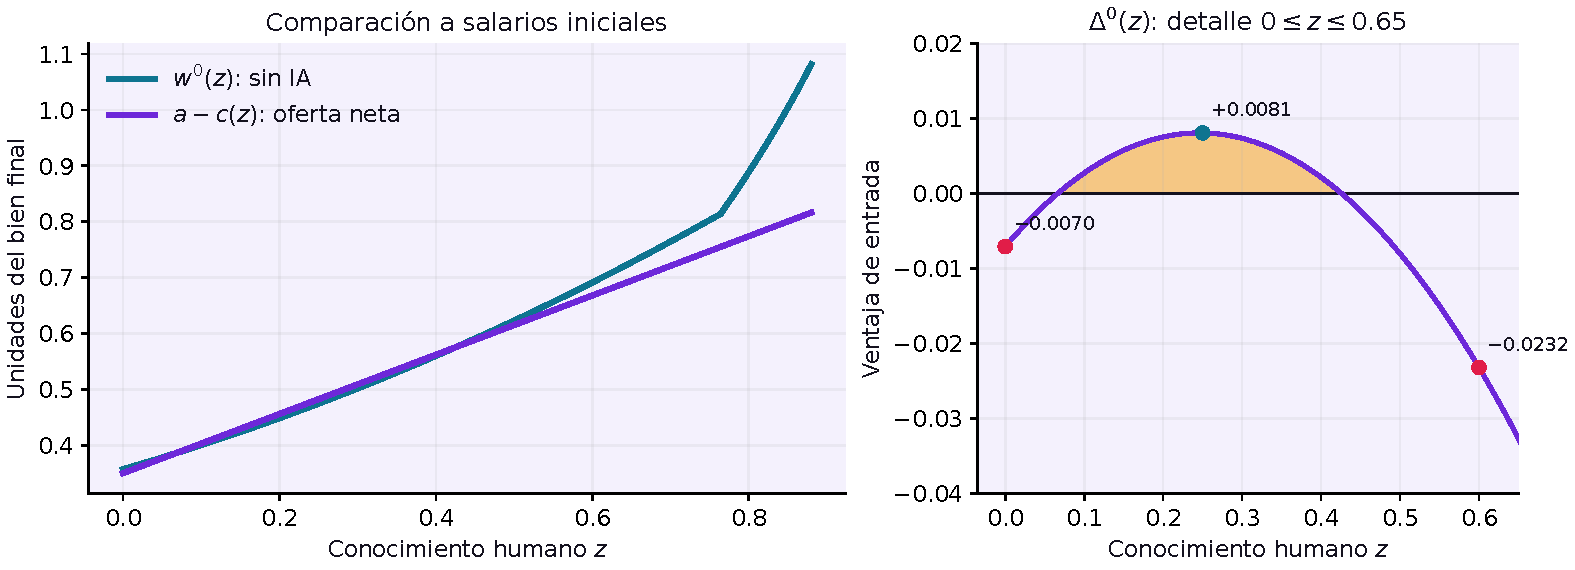
\includegraphics[width=.90\linewidth]{../code/figures/entry_check.pdf}
\small
\begin{tabular}{rrrr}\toprule
$z$ & $w^0(z)$ & $a-c(z)$ & $\Delta^0(z)$\\\midrule
0.00&0.3570&0.3500&$-0.0070$\\
0.25&0.4744&0.4825&$+0.0081$\\
0.60&0.6912&0.6680&$-0.0232$\\\bottomrule
\end{tabular}
\sourcefoot{Cálculo propio: $G(z)=z$, $h=0.5$, $a=0.88$, $\kappa=0.53$. code/verify.py. Entrada a salarios iniciales; no es equilibrio.}
\end{frame}
\section{Por qué no está resuelto}
% 11: 1:00
\begin{frame}{4. Por qué no está resuelto: dentro del paper}
\begin{itemize}
\item \textbf{Apéndice, sección 2.6:} la prueba utiliza salarios iguales entre usuarios de IA. Con $c(z)$, ese paso debe revisarse.
\item \textbf{Versiones v1--v12:} v7 modela otra forma de no autonomía; v8--v10 tienen la Proposición 7; v11--v12, la Proposición 6.
\item \textbf{Capítulo 5 del apéndice:} estudia otras consecuencias y cómputo escaso, sin este gasto real por tipo.
\end{itemize}
\begin{keybox}
Extender requiere re-derivar el ordenamiento. Un salario inclinado no demuestra por sí solo que el orden se invierta.
\end{keybox}
\sourcefoot{Apéndice, pp. impresas 21--23 y 64--74; registro: proposal/literature-search.md.}
\end{frame}
% 12: 1:30
\begin{frame}{4. Por qué no está resuelto: literatura cercana}
\small
\begin{tabular}{@{}p{.29\linewidth}p{.64\linewidth}@{}}\toprule
Trabajo y estado & Qué hace y cómo se diferencia\\\midrule
Xu et al. (2025)\newline Preprint & Validación gerencial consume tiempo y elimina alucinaciones. Aquí: gasto real por tipo y tecnología fija.\\[5pt]
Quispe y Xu (2026)\newline Preprint v2 & Costo de verificación decreciente con habilidad; banda de lenguajes. Aquí: tipos humanos, salarios y jerarquías en equilibrio.\\[5pt]
Catalini et al. (2026)\newline Preprint & Verificación y experiencia con salario experto; no cierra este mercado laboral.\\[5pt]
Ide y Talamàs, Turing Valley\newline Aceptado: J. Human Capital & Heterogeneidad y sinergias; no esta fricción en la Proposición 6.\\\bottomrule
\end{tabular}
\medskip
\textbf{Novedad provisional:} caracterizar la adopción en este equilibrio. Scholar ``Citado por'' y arXiv revisados; Semantic Scholar: límite 429.
\sourcefoot{Fuentes y alcance en proposal/literature-search.md; referencias en apéndice C.}
\end{frame}
\section{Plan y riesgos}
% 13: 2:00. Total central: 20 minutos.
\begin{frame}{5. Plan y riesgos}
\begin{columns}[T]
\column{.55\textwidth}
\textbf{Probar}\par
Usuarios de IA; recuperar Prop. 6 con $c=0$; costo constante frente a pendiente.
\medskip\par
\textbf{Simular}\par
Adaptar el LP con producto neto $a-c(z)$; factibilidad, dualidad y refinamiento de malla.
\medskip\par
\textbf{Formalizar en Lean}\par
FOC, $w^V=a-c$ y la futura proposición sobre adoptantes, con AppliedModelingLib.
\column{.41\textwidth}
\begin{block}{Mayor riesgo}
Existencia/unicidad del equilibrio continuo y supervivencia de la selección intermedia tras la reasignación.
\end{block}
\textbf{Plan B:} modelo discreto de dos o tres tipos.
\medskip\par
Hoy: álgebra y entrada verificadas.\par
Equilibrio y Lean: pendientes.
\end{columns}
\sourcefoot{Extensión propia: no atribuyo un error al paper. Final: 28-oct; paper: 26-nov.}
\end{frame}
\appendix
\begin{frame}{A. Condiciones locales y fronteras}
\[\Pi^{V\prime}(0)\leq0,\qquad\Pi^{V\prime}(a)\geq0\]
Condiciones necesarias unilaterales si el óptimo está en un extremo.
\medskip
En un punto estacionario dos veces diferenciable, como
$n''=2n'/(1-z)$, la FOC cancela los términos de escala:
\[\Pi^{V\prime\prime}(z)=-n(z)[w^{V\prime\prime}(z)+c''(z)].\]
Para un máximo local se requiere $\Pi^{V\prime\prime}\leq0$.
\begin{keybox}
Con salario de beneficio cero y costo lineal, puede haber indiferencia. No hay un $z$ óptimo único deducible de la FOC.
\end{keybox}
\end{frame}
\begin{frame}{B. Lo que falta para cerrar el equilibrio}
\begin{itemize}
\item Ninguna actividad puede dar beneficios positivos a salarios $w^V$.
\item Actividades efectivamente usadas: beneficio cero.
\item Recursos humanos factibles y mercados que se vacían.
\item Cómputo: demanda factible, $r\geq0$ y complementariedad.
\end{itemize}
\[w^V(z)\geq z,\qquad w^V(z)\geq a-c(z)\quad(z\leq a),\]
\[w^V(z)+h(1-z)w^V(s)\geq s\quad(0\leq z\leq s\leq1).\]
\small Igualdad en actividades usadas. El nuevo salario debe satisfacer todas las opciones; no se reemplaza mecánicamente por $w^0$.
\end{frame}
\begin{frame}{C. Referencias y reproducción}
\footnotesize
\begin{itemize}
\item Ide y Talamàs (2025), \emph{Artificial Intelligence in the Knowledge Economy}. JPE 133(12), 3762--3800. \href{https://doi.org/10.1086/737233}{DOI 10.1086/737233}; \href{https://arxiv.org/abs/2312.05481v11}{arXiv v11}, Prop. 6, p. 27.
\item \href{https://www.eduardtalamas.com/}{Apéndice en la web del autor}, 23-feb-2025; pp. impresas 21--23 y 64--74.
\item Xu, Hou, Chen y Xie (2025), \emph{Generative AI and Organizational Structure in the Knowledge Economy}. \href{https://arxiv.org/abs/2506.00532v1}{arXiv:2506.00532v1}, sec. 5; preprint.
\item Quispe y Xu (2026), \emph{Agentic Delegation and the Language Frontier of Software Developers}. \href{https://arxiv.org/abs/2605.25438v2}{arXiv:2605.25438v2}, sec. 4; preprint.
\item Catalini, Hui y Wu (2026), \emph{Some Simple Economics of AGI}. \href{https://arxiv.org/abs/2602.20946v1}{arXiv:2602.20946v1}, sec. 3.4.1 y 5.2; preprint.
\item Ide y Talamàs, \emph{The Turing Valley}. \href{https://arxiv.org/abs/2408.16443}{arXiv:2408.16443}; aceptado en J. Human Capital según web del autor.
\end{itemize}
\medskip
\texttt{python3 code/verify.py} reproduce la tabla y figura.\par
Búsquedas: \texttt{proposal/literature-search.md}. Guion: \texttt{slides/guion-topic.md}.
\end{frame}
\end{document}
